\documentclass[11pt]{article}
%基于北京航空航天大学仪器科学与光电工程学院实验报告及课程报告排版得来,类似于毕业论文排版格式
%后续将更新毕业论文排版格式
\usepackage{graphicx,float}%使用图的宏包,使用图的浮动体宏包,引入参数H使图像紧跟当前文字
\usepackage{caption} %使用图表标题的宏包
\usepackage[colorlinks=true,pdfstartview=FitH,%
linkcolor=black,anchorcolor=violet,citecolor=magenta]{hyperref}%加载hyperref宏包,使用超链接
\usepackage{setspace}%用于设置行间距列间距等命令的宏包
\usepackage{array}%设置列表高度宽度的宏包
\usepackage{zhnumber}%使用中文数字编号的宏包
\usepackage{titlesec,titletoc}%使用标题自定义形式的宏包和使用目录自定义形式的宏包
\usepackage{siunitx}%物理学单位宏包
\usepackage{tabularx}%让表格宽度等于页面宽度
\usepackage{makecell}%单个表格单元调整的宏包
\usepackage{subfigure} %%使用子图的宏包
\usepackage[backend=biber,bibstyle=gb7714-1987,%nature,%%加载biblatex宏包,使用参考文献
citestyle=gb7714-1987%,backref=true%%其中后端backend使用biber
,url=false
]{biblatex}%标注(引用)样式citestyle,著录样式bibstyle都采用gb7714-2015样式
% \usepackage{pgfplots}%类似tikz的一个画图库,主要画统计图
\usepackage{../customStyle}
% \usepackage{customFont}%自行编写的字体命令库,基于CJK宏包
% \usepackage{bh_style}%自行编写的风格文件,基于使用习惯和格式要求
% \usepackage{math_formulate}%自行编写的数学公式命令库,基于amsmath宏包
% \usepackage{picture}%集成图形绘制库,主要包括了tikz和pgfplots两大主流宏包
% \usepackage[lite,subscriptcorrection,slantedGreek,nofontinfo]{mtpro2}%使用mathtimepro2商业字体作为数学环境,并不推荐

%biblatex宏包的参考文献数据源加载方式,注意book.bib应当与.tex文件在同一目录下,不然有可能会报错
\addbibresource[location=local]{book.bib}
% % \bibliographystyle{gbt7714-numerical}
%%% 下面的命令重定义页面边距,使其符合中文刊物习惯 %%%%
% \addtolength{\topmargin}{2.5cm}
\setlength{\oddsidemargin}{0.63cm}  % 3.17cm - 1 inch
\setlength{\evensidemargin}{\oddsidemargin}
% \setlength{\textwidth}{14.66cm}
% \setlength{\textheight}{24.00cm}    % 24.62

\graphicspath{{./fig}}

\begin{document}
\section{多视图几何知识点}
\subsection{齐次坐标二维点、二维线的表示,齐次坐标二维点和线的关系(相交、点在线上、交点交线)P20}
设齐次点为$\mathbf{x}=(x_1,x_2,x_3)^T$,齐次线为$\mathbf{l}=(l_1,l_2,l_3)^T$,其中点和线都是二维的,则从齐次点退化为非齐次点可用下式:
\begin{equation*}
  \mathbf{x}=(x_1,x_2,x_3)^T=\circbrac{\frac{x_1}{x_3},\frac{x_2}{x_3}}^T
\end{equation*}\par
点在直线上:
\begin{equation*}
  \mathbf{x}^T\mathbf{l}=0
\end{equation*}\par
两个齐次点确定一条直线:
\begin{equation*}
  \mathbf{l}=\mathbf{x}\times\mathbf{x}'
\end{equation*}\par
两条齐次线确定一个点:
\begin{equation*}
  \mathbf{x}=\mathbf{l}\times\mathbf{l}'
\end{equation*}\par
\subsection{什么是理想点?P21}
理想点就是位于无穷远直线或者无穷远平面上的点,又称消隐点,其齐次坐标的最后一个坐标值为0。
\subsection{二维二次曲线的表示、对偶二次曲线与二次曲线的关系,二次曲线切线切点怎么表示?P23}
二维二次曲线的表示:
\begin{equation*}
  \mathbf{C}=\begin{bmatrix}
    a   & b/2 & d/2 \\
    b/2 & c   & e/2 \\
    d/2 & e/2 & f
  \end{bmatrix}
\end{equation*}\par
点在二次曲线上的表示:
\begin{equation*}
  \mathbf{x}^T\mathbf{C}\mathbf{x}=0
\end{equation*}\par
对偶二次曲线:二次曲线上的全部切线所形成的包络,即符合以下公式:
\begin{equation*}
  \mathbf{l}^T\mathbf{C}^*\mathbf{l}=0
\end{equation*}\par
对偶二次曲线等于二次曲线的伴随矩阵,当二次曲线可逆时,该伴随矩阵在齐次意义下等于二次曲线的逆矩阵。\par
经过二次曲线上某一点的切线可表示为:
\begin{equation*}
  \mathbf{l=Cx}
\end{equation*}
\subsection{退化二次曲线P24}
退化二次曲线是不满秩的二次曲线,当秩为2时,可以表示为两条直线的乘积,即:
\begin{equation*}
  \mathbf{C}=\mathbf{ml}^T+\mathbf{lm}^T
\end{equation*}\par
当秩为1时,二次曲线退化为一个重合的点。
\subsection{二次曲线极点-极线关系、共轭概念、仿射分类P44}
二次曲线外一点$\mathbf{x}$可作二次曲线两条切线$\mathbf{l}_1,\mathbf{l}_2$,两切点$\mathbf{x}_1,\mathbf{x}_2$确定一条直线$\mathbf{l}=\mathbf{l_1}\times\mathbf{l}_2$,该直线称为极线,点$\mathbf{x}$称为极点,二者具有以下的关系:
\begin{equation*}
  \mathbf{l}=\mathbf{Cx}
\end{equation*}\par
因此又有以下的关系,称为共轭关系:
\begin{equation*}
  \mathbf{l}^T\mathbf{C}\mathbf{x}=0
\end{equation*}\par
二次曲线根据其仿射性质可以分为三类,如下表:
\begin{table}[H]
  \centering
  \caption{二次曲线的仿射分类}
  \begin{tabular}{|c|c|c|c|}
    \hline
    二次曲线 & 圆(椭圆) & 抛物线 & 双曲线 \\
    \hline
    与无穷远直线交点 & 0个 & 1个 & 2个 \\
    \hline
  \end{tabular}
\end{table}
\subsection{点变换、直线协变、二次曲线协变、对偶二次曲线逆变P27}
在单应$\mathbf{H}$作用下,点$\mathbf{x}$变换为$\mathbf{x}'$,则有:
\begin{equation*}
  \mathbf{x}'=\mathbf{Hx} 
\end{equation*}\par
直线$\mathbf{l}$变换为$\mathbf{l}'$,则有:
\begin{equation*}
  \mathbf{l}'=\mathbf{H}^{-T}\mathbf{l}
\end{equation*}\par
二次曲线$\mathbf{C}$变换为$\mathbf{C}'$,则有:
\begin{equation*}
  \mathbf{C}'=\mathbf{H}^{-T}\mathbf{CH}^{-1}
\end{equation*}\par
对偶二次曲线$\mathbf{C}^*$变换为$\mathbf{C}^{*'}$,则有:
\begin{equation*}
  \mathbf{C}^{*'}=\mathbf{HC}^*\mathbf{H}^T
\end{equation*}\par
由于直线和二次曲线的变换中含有$\mathbf{H}^{-1}$项,因此又称为协变。
\subsection{四类变换的性质及其变换矩阵P30}
欧氏变换,又称刚体变换,不改变原始形状的长度和夹角,其变换矩阵为:
\begin{equation*}
  \mathbf{H}=\begin{bmatrix}
    \mathbf{R} & \mathbf{t} \\
    \mathbf{0}^T & 1
  \end{bmatrix} 
\end{equation*}\par
其中,$\mathbf{R}$为旋转矩阵,$\mathbf{t}$为平移向量。\par
相似变换,又称等距变换,不改变原始形状的夹角,其变换矩阵为:
\begin{equation*}
  \mathbf{H}=\begin{bmatrix}
    s\mathbf{R} & \mathbf{t} \\
    \mathbf{0}^T & s
  \end{bmatrix}
\end{equation*}\par
其中增加了一项缩放因子$s$,是对整个图像的均匀缩放。\par
仿射变换,不改变原始形状的平行性,变换矩阵为:
\begin{equation*}
  \mathbf{H}=\begin{bmatrix}
    \mathbf{A} & \mathbf{t} \\
    \mathbf{0}^T & 1
  \end{bmatrix}
\end{equation*}\par
其中矩阵$\mathbf{A}$是一个非奇异的矩阵。\par
射影变换,不改变原始形状的直线性,变换矩阵为:
\begin{equation*}
  \mathbf{H}=\begin{bmatrix}
    \mathbf{A} & \mathbf{t} \\
    \mathbf{v}^T & 1
  \end{bmatrix}
\end{equation*}\par
其中矩阵$\mathbf{A}$是一个非奇异的矩阵,向量$\mathbf{v}$是非零向量。
\subsection{	射影变换阵的分解P32}
射影矩阵可以分解为三个独立的变换,即:
\begin{equation*}
  \mathbf{H}=\begin{bmatrix}
    s\mathbf{R} & \mathbf{t} \\
    \mathbf{0}^T & 1
  \end{bmatrix}
  \begin{bmatrix}
    \mathbf{K} & \mathbf{0} \\
    \mathbf{0}^T & 1
  \end{bmatrix}
  \begin{bmatrix}
    \mathbf{I} & \mathbf{0} \\
    \mathbf{v}^T & 1
  \end{bmatrix}
  \triangleq\mathbf{H}_S\mathbf{H}_A\mathbf{H}_P
\end{equation*}\par
其中,$\mathbf{H}_P$仅改变图像的无穷远直线(射影变换),$\mathbf{H}_A$是仅改变比例尺的长宽比(仿射变换),$\mathbf{H}_S$是相似变换。\par
射影变换的逆变换矩阵也是一个射影变换,因此也可以分解成类似的结果,通常将它们反着写,即:
\begin{equation*}
  \mathbf{H}'=\mathbf{H}'_P\mathbf{H}'_A\mathbf{H}'_S
\end{equation*}\par
\subsection{	两种恢复至仿射变换的方法P37}
恢复至仿射变换,需要将无穷远直线校正至规范位置,因此需要求出图像的无穷远直线即可:
\begin{itemize}
  \item 通过两对平行线的交点求出无穷远直线;
  \item 通过交比不变,作图求出无穷远直线。
\end{itemize}
\subsection{三种恢复至相似变换的方法P41}
恢复至仿射变换,需要将绝对对偶二次曲线校正至规范位置,因此需要求出绝对对偶二次曲线:
\begin{itemize}
  \item 通过五正交直线;
  \item 在仿射校正的基础上,通过两对正交直线即可校正;
  \item 在仿射校正的基础上,通过一个椭圆或者一个已知长度的交比来计算校正。
\end{itemize}
\subsection{三维点和平面的齐次式以及关联定义、对偶定义,平面点的参数方程表示P50}
三维点定义:$\mathbf{X}=(X_1,X_2,X_3,X_4)^T$,平面定义为:$\mathbold{\pi}=(\pi_1,\pi_2,\pi_3,\pi_4)^T$,点在平面上,可有以下关系:
\begin{equation*}
  \mathbold{\pi}^T\mathbf{X}=0
\end{equation*}\par
平面点的参数方程表示:
\begin{equation*}
  \mathbf{X}=\mathbf{Mx}
\end{equation*}\par
式中,$\mathbf{M}$是平面$\mathbold{\pi}$的零空间,是一个$4\times3$的矩阵,$\mathbf{x}$是一个三维齐次向量,即参数。
\subsection{	空间直线的生成子空间表示和零空间表示、平面与直线的交点以及包含一条直线和点的平面定义方法P52}
两个空间点构成矩阵:
\begin{equation*}
  \begin{bmatrix}
    \mathbf{X}_1^T \\
     \mathbf{X}_2^T
  \end{bmatrix} 
\end{equation*}\par
空间直线是它的生成子空间,即:
\begin{equation*}
  \mathbf{X}=\lambda_1\mathbf{X}_1+\lambda_2\mathbf{X}_2
\end{equation*}\par
空间直线也可以使用两个平面的零空间表示,即:
\begin{equation*}
  \begin{bmatrix}
    \mathbold{\pi}_1^T \\
     \mathbold{\pi}_2^T
  \end{bmatrix} \mathbf{l}=0
\end{equation*}\par
平面与直线的交点,相当于三个平面交于一点,需要使用零空间表示,即:
\begin{equation*}
  \begin{bmatrix}
    \mathbold{\pi}_1^T \\
    \mathbold{\pi}_2^T\\
    \mathbold{\pi}_3^T
  \end{bmatrix} \mathbf{X}=0
\end{equation*}\par
直线与一点共面,相当于三个点位于平面上,需要使用生成子空间表示 ,即:
\begin{equation*}
  \begin{bmatrix}
    \mathbf{X}_1^T \\
    \mathbf{X}_2^T\\
    \mathbf{X}_3^T
  \end{bmatrix} \mathbold{\pi}=0
\end{equation*}\par
\subsection{使用Plücker矩阵定义的直线以及对偶直线,直线和平面的关联P53}
直线的Plücker矩阵定义(下文中全部大写的L均表示Plücker形式的直线):
\begin{equation*}
  \mathbf{L}=\mathbf{X}_1\mathbf{X}_2^T-\mathbf{X}_2\mathbf{X}_1^T
\end{equation*}\par
对偶直线的Plücker矩阵定义:
\begin{equation*}
  \mathbf{L}^*=\mathbold{\pi}_1\mathbold{\pi}_2^T-\mathbold{\pi}_2\mathbold{\pi}_1^T
\end{equation*}\par
直线与平面交于一点,即:
\begin{equation*}
  \mathbf{X}=\mathbf{L}^T\mathbold{\pi}
\end{equation*}\par
直线和一点共面,即:
\begin{equation*}
  \mathbold{\pi}=\mathbf{L}^T\mathbf{X}
\end{equation*}\par
\subsection{两直线相交的充要条件以及三个推论P54}
两直线相交的充要条件是两直线的双线性乘积为零,即:
\begin{equation*}
  \mathcal{L_1|L_2}=\det\circbrac{\mathbf{X}_1,\mathbf{X}_2,\mathbf{X}_3,\mathbf{X}_4}=0
\end{equation*}\par
三个推论分别是:
\begin{itemize}
  \item 一条直线和另一条直线的对偶形式已知,则可以写出:\\
  $\circbrac{\mathbold{\pi}_1^T\mathbf{X}_1}\cdot\circbrac{\mathbold{\pi}_2^T\mathbf{X}_2}-\circbrac{\mathbold{\pi}_2^T\mathbf{X}_1}\cdot\circbrac{\mathbold{\pi}_1^T\mathbf{X}_2}=0$
  \item 使用两平面表示的直线也可以得到相同的双线性乘积结果:\\
  $\mathcal{L_1|L_2}=\det\circbrac{\mathbold{\pi}_1,\mathbold{\pi}_2,\mathbold{\pi}_3,\mathbold{\pi}_4}=0
  $
  \item 六维向量$\mathcal{L}=[l_12,l_12,l_14,l_23,l_24,l_34]^T$仅表示一条三维直线,当且仅当双线性乘积为零。
\end{itemize}
\subsection{	绝对二次曲线、度量两空间直线的夹角,四个关于绝对二次曲线的性质P61}
绝对二次曲线定义为符合以下公式的全部点的集合:
\begin{align*}
  \left\{
    \begin{aligned}
      x_1^2+x_2^2+x_3^2&=0\\
      x_4&=0
    \end{aligned}
  \right.
\end{align*}\par
在规范位置处,绝对二次曲线可以表示为:
\begin{equation*}
  \mathbold{\Omega}_\infty=\begin{bmatrix}
    1 & 0 & 0 & 0 \\
    0 & 1 & 0 & 0 \\
    0 & 0 & 1 & 0 \\
    0 & 0 & 0 & 0
  \end{bmatrix}
\end{equation*}\par
求解两空间直线的夹角,可以使用以下公式:
\begin{equation*}
  \cos\theta=\frac{\mathbf{L}_1^T\mathbold{\Omega}_\infty\mathbf{L}_2}{\sqrt{\mathbf{L}_1^T\mathbold{\Omega}_\infty\mathbf{L}_1}\sqrt{\mathbf{L}_2^T\mathbold{\Omega}_\infty\mathbf{L}_2}}
\end{equation*}\par
四点关于绝对二次曲线的性质:
\begin{itemize}
  \item 绝对二次曲线与直线交于两个虚球点;
  \item 绝对二次曲线与任意的圆交于两个虚球点;
  \item 绝对二次曲线与任意的球交于无穷远平面;
  \item 绝对二次曲线在相似变换作用下保持集合不变,而不是点点不变。
\end{itemize}
\subsection{绝对对偶二次曲面、度量两平面夹角P63}
绝对对偶二次曲面是绝对二次曲线全部切平面的包络,表示为:
\begin{equation*}
  \mathbf{Q}^*_\infty=\begin{bmatrix}
    1 & 0 & 0 & 0 \\
    0 & 1 & 0 & 0 \\
    0 & 0 & 1 & 0 \\
    0 & 0 & 0 & 0
  \end{bmatrix}
\end{equation*}\par
度量两平面的夹角,可以使用以下公式:
\begin{equation*}
  \cos\theta=\frac{\mathbold{\pi}_1^T\mathbf{Q}^*_\infty\mathbold{\pi}_2}{\sqrt{\mathbold{\pi}_1^T\mathbf{Q}^*_\infty\mathbold{\pi}_1}\sqrt{\mathbold{\pi}_2^T\mathbf{Q}^*_\infty\mathbold{\pi}_2}}
\end{equation*}\par
绝对对偶二次曲面在相似变换下保持不变。
\subsection{摄像机的中心、图像平面、主轴、主点、主平面P117}
投影中心称为摄像机的中心,记为$\mathbf{C}$;\par
摄像机的主轴定义为,过摄像机中心且与摄像机光轴平行的矢量方向;\par
图像平面定义为,与摄像机中心保持焦距位置处,与主轴垂直的平面;\par
摄像机的主点定义为,摄像机主轴与图像平面的交点;\par
摄像机的主平面定义为,经过摄像机\textbf{中心}且与摄像机主轴垂直的平面。\par
\subsection{摄像机投影矩阵P的四种写法、内参数和外参数P118}
摄像机投影矩阵可以写为以下四种形式:
\begin{itemize}
  \item 标准形式(世界坐标系与相机坐标系重合):$\mathbf{P}=\mathbf{K[I|0]}$;
  \item 当世界坐标系与相机坐标系不重合时,使用相机的中心表示为:$\mathbf{P}=\mathbf{K[R|-R\tilde{C}]}$;
  \item 将内参数矩阵和外参数矩阵分离的形式,写为:$\mathbf{P}=\mathbf{KR}\mathbf{[I|-\tilde{C}]}$;
  \item 保留最后一列的形式:$\mathbf{P}=\mathbf{M}\mathbf{[I|M^{-1}p_4]}$。
\end{itemize}\par
第二种形式给出了内参数和外参数的定义,内参数矩阵为:$\mathbf{K}$;外参数矩阵为$\mathbf{[R|t]}$。
\subsection{解读标定矩阵P,摄像机中心、列向量含义、行向量含义、主平面、轴平面、主点以及主射线的数学表示P121}
记标定矩阵$\mathbf{P}$为:
\begin{equation*}
  \mathbf{P}=\begin{bmatrix}
    P_1^T\\\\
    P_2^T\\\\
    P_3^T
  \end{bmatrix}
  =\begin{bmatrix}
    p_1&p_2&p_3&p_4
  \end{bmatrix}=\begin{bmatrix}
    p_{11}&p_{12}&p_{13}&p_{14}\\
    p_{21}&p_{22}&p_{23}&p_{24}\\
    p_{31}&p_{32}&p_{33}&p_{34}
  \end{bmatrix}
\end{equation*}\par
投影矩阵的行向量$P_1^T,P_2^T$代表图像上x轴和y轴的与相机主轴形成的两个平面,称为轴平面;第三行$P_3^T$代表相机的主平面;\par
投影矩阵的列向量$p_1,p_2,p_3$代表相机对世界坐标系x轴、y轴、z轴成像所得到的像点;第四列向量$p_4$代表相机对世界坐标系坐标原点的图像;\par
相机的中心是两个轴平面与主平面的交点,因此可以使用标定矩阵$\mathbf{P}$的零空间来表示:$\mathbf{C}=\mathcal{N}(\mathbf{P})$;\par
摄像机的主点是主轴向量对主平面的交点,主轴向量是主平面的法向量,因此是投影矩阵第三行的无穷远点,即$[p_{31},p_{32},p_{33},0]^T$,相机对该无穷远点成像即为主点,书上取前三项为$m_3$,因此简写为$\mathbf{M}m_3$;\par
相机的主射线是主平面正向的方向,摄像机主点中$m_3$提供了方向,但是不包含正负号,因此主轴方向上指向摄像机前方的向量为$\det(\mathbf{M})m_3$。
\subsection{	仿射摄像机P矩阵的特点P127}
仿射摄像机相当于对有限摄像机的焦距调整至无穷大,同时将相机置于无穷远处,因此其主平面位于无穷远平面,标定矩阵最后一行为$[0,0,0,1]$。
\subsection{仿射摄像机与有限摄像机的三个区别P131}
\begin{itemize}
  \item 平行投影矩阵$\begin{bmatrix}
    1&0&0&0\\
    0&1&0&0\\
    0&0&0&1
  \end{bmatrix}$代替了有限摄像机的规范射影矩阵$\mathbf{[I|0]}$;
  \item 标定矩阵$\begin{bmatrix}
    K_{2\times2}&0\\
    0^T&1
  \end{bmatrix}$代替了有限摄像机的上三角阵$\mathbf{K}$;
  \item 主点位于无穷远处,即主点无定义。
\end{itemize}
\subsection{摄像机将二次曲线反向投影成锥面、将二次曲面映射为二次曲线P153}
对于某个图像上的二次曲线$\mathbf{Q}$,其在空间中的反向投影为$\mathbf{Q}'=\mathbf{P}^T\mathbf{QP}$,证明该反向投影为锥面(即不满秩):由于$\mathbf{PC}=0$,对反向投影右乘摄像机中心坐标可得:$\mathbf{Q}'\mathbf{C}=\mathbf{P}^T\mathbf{QPC}=0$,即矩阵$\mathbf{Q}'$一定是不满秩的,因此该反向投影是锥面。\par
摄像机将二次曲面映射为二次曲线,即:???
\subsection{摄像机同中心缩放、纯旋转的单应矩阵P156}
摄像机同中心缩放,相当于其左乘一个倍缩变换矩阵,即有:
\begin{equation*}
  \mathbf{P}'=\begin{bmatrix}
    s&0&0\\
    0&s&0\\
    0&0&1
  \end{bmatrix}\mathbf{P}
\end{equation*}\par
摄像机同中心纯旋转,相当于对世界坐标系乘以一个旋转矩阵,即:
\begin{equation*}
  \mathbf{P}'=\mathbf{PR}
\end{equation*}\par
\subsection{摄像机标定矩阵$\mathbf{K}$是图像点与欧氏坐标系下的射线方向的一个单应(仿射变换)P161}
不知道怎么证?
\subsection{三维空间的消影点在图像的位置P165}
三维空间的无穷远平面在图像平面上成像为无穷远直线。
\subsection{对极点、对极平面和对极线的概念P185}
两个摄像机的中心与空间中一点形成的平面称为对极平面;中心的连线与图像平面的交点称为对极点;两个摄像机各自图像平面与对极平面的交线称为对极线。
\subsection{基本矩阵的四项几何含义P189}
基本矩阵有多种表现形式,以下根据要求写出几种:
\begin{equation*}
  \mathbf{F}=
\end{equation*}


\section{简答证明要点}
\subsection{证明射影变换交比不变}
方法一:三角形面积法,即证明三角形面积的比值不变;\par
方法二:使用齐次坐标,如下图:
\begin{figure}[H]
  \centering
  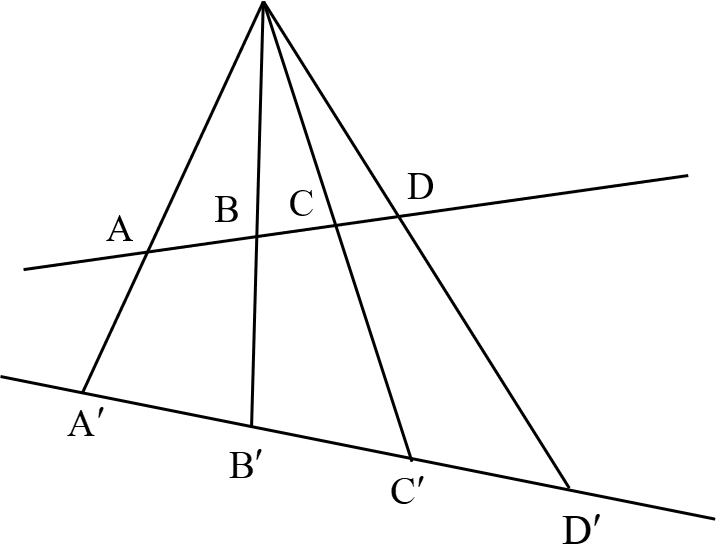
\includegraphics[width=0.5\linewidth]{证明题1.png}
  \caption{射影变换交比不变证明}
\end{figure}\par
交比定义为距离比的比值,在一维空间中的齐次坐标系下,可以使用行列式表示:
$$
\mathrm{Cross}(A,B,C,D)=\frac{
  |AC||AD|
}{|BC||BD|}
$$\par
式中,
$$
|AC|=\det\begin{bmatrix}
  x_A & x_C  \\
  y_A& y_C  \\
\end{bmatrix}
$$\par
是前两项的行列式,因此可设:
$$
\begin{aligned}
\mathbf{A}'=s_1\mathbf{HA}\\
\mathbf{B}'=s_2\mathbf{HB}\\
\mathbf{C}'=s_3\mathbf{HC}\\
\mathbf{D}'=s_4\mathbf{HD}
\end{aligned}
$$\par
代入行列式中,得:
$$
\begin{aligned}
|A'B'|=\det\begin{bmatrix}
  s_1\mathbf{HA}& s_2\mathbf{HB}  
\end{bmatrix}=s_1s_2\det(\mathbf{H})|AB|
\end{aligned}
$$\par
同理可得:
$$
\begin{aligned}
|A'C'|=s_1s_3\det(\mathbf{H})|AC|\\
|A'D'|=s_1s_4\det(\mathbf{H})|AD|\\
|B'C'|=s_2s_3\det(\mathbf{H})|BC|\\
|B'D'|=s_2s_4\det(\mathbf{H})|BD|\\
\end{aligned}
$$\par
代入交比定义,即可验证四个比例因子和行列式$\det\mathbf{H}$均被消去,原式得证。
\subsection{证明仿射变换能把圆映射成椭圆但是不能映射成双曲线和抛物线}
根据二次曲线的仿射分类可知,与无穷远直线没有交点的二次曲线是椭圆或者圆,有一个交点的二次曲线是抛物线,有两个交点的二次曲线是双曲线。仿射变换不改变无穷远直线,而交点性质是射影变换都不会改变的,因此经过仿射变换后,曲线与无穷远直线的交点数量不会变化,所以圆不会变成双曲线和抛物线,而可能变成椭圆。
\subsection{证明仿射变换下平行的两条线段长度之比不变,而不平行的则不然}
设平行线段$AB$和$CD$,则有:
$$
\begin{aligned}
\mathbf{A-B}=&\lambda(\mathbf{C-D})\\
\frac{|AB|}{|CD|}=&\lambda
\label{eq:证明题3}
\end{aligned}
$$\par
其中$\lambda$为常数,设仿射变换为$\mathbf{X}'=\mathbf{HX}$,则有:
$$
\mathbf{H}=\begin{bmatrix}
  \mathbf{A}& \mathbf{v}\\
   0&1\\
\end{bmatrix}
$$\par
当平行线段的端点ABCD不含有无穷远点时,经过仿射变换后,有:
$$
\begin{aligned}
\mathbf{A}'=\begin{bmatrix}
\mathbf{AX}_A+\mathbf{v}z_A\\
z_A
\end{bmatrix}
\end{aligned}
$$\par
因此两平行线段的长度相应地变化为:
$$
\begin{aligned}
|A'B'|=&\sqrt{(\mathbf{X}_A-\mathbf{X}_B)^T\mathbf{A}^T\mathbf{A}(\mathbf{X}_A-\mathbf{X}_B)}\\
|C'D'|=&\sqrt{(\mathbf{X}_C-\mathbf{X}_D)^T\mathbf{A}^T\mathbf{A}(\mathbf{X}_C-\mathbf{X}_D)}\\
=&\lambda\sqrt{(\mathbf{X}_A-\mathbf{X}_B)^T\mathbf{A}^T\mathbf{A}(\mathbf{X}_A-\mathbf{X}_B)}\\
\end{aligned}
$$\par
因此两线段长度之比不变。对于不平行的线段,由于公式\ref{eq:证明题3}不成立,因此其长度之比不能保持不变。
\end{document}